\documentclass{beamer}
\usepackage{ulem}
\usepackage{tikz}
\usepackage{booktabs}
\usepackage{graphicx,threeparttable,caption}
\usetikzlibrary{shapes,snakes}
\usepackage[beamer,customcolors]{hf-tikz}
\usepackage{nicematrix}
\usepackage{xcolor}
\usepackage{makecell}
\usepackage{array}
\usepackage{csquotes}
\usepackage{csquotes}
\usepackage{minted}
\usepackage{animate}
\captionsetup{labelformat=empty,labelsep=none}

\graphicspath{ {./png/} }

\usetikzlibrary{
    arrows,
    arrows.meta,
    shapes,
    positioning,
    shadows,
    trees,
    calc
}

\tikzset{%
    >={Latex[width=2mm,length=2mm]},
    % Specifications for style of nodes:
    plain/.style = {},
    base/.style = {
        plain,
        rectangle, rounded corners, draw=black,
        minimum width=1cm, minimum height=1cm,
        text centered, font=\sffamily\tiny\bfseries,
        fill=white, align=center
    },
    app/.style = {base, ellipse},
    data/.style = {base, fill=gray!30},
    action/.style = {base, circle, fill=red!30},
    note/.style = {app, fill=yellow},
    hl/.style={
    set fill color=red!80!black!40,
    set border color=red!80!black
    }
}


\AtBeginSection[]{
  \begin{frame}
  \vfill
  \centering
  \begin{beamercolorbox}[sep=8pt,center,shadow=true,rounded=true]{title}
    \usebeamerfont{title}\insertsectionhead\par%
  \end{beamercolorbox}
  \vfill
  \end{frame}
}
\setbeamercolor{alerted text}{fg=red}
%\usecolortheme[orchid]{structure}
\usetheme[hideothersubsections]{PaloAlto}
\makeatletter
\patchcmd{\csq@bquote@i}{{#6}}{{\emph{#6}}}{}{}
\makeatother
%\usecolortheme{orchid}
%\usefonttheme{professionalfonts}
\newcommand{\soutthick}[1]{%
   \textcolor{red}{
   \renewcommand{\ULthickness}{1pt}%
      \sout{#1}%
   \renewcommand{\ULthickness}{.4pt}% Resetting to ulem default
   }
}
\newcommand{\centered}[1]{\begin{tabular}{l} #1 \end{tabular}}
\setbeamertemplate{section in toc}[square]
\setbeamertemplate{subsection in toc}[square]
\setbeamertemplate{section in sidebar}[shaded]
\setbeamertemplate{items}[square]
\setbeamercovered{transparent} 

\title[]{Introduction to Computational Social Science}
\subtitle{Working with the GDELT API}
\author[]{Mikołaj Biesaga\\ \small{\color{blue}{\href{mailto:m.biesaga@uw.edu.pl}{m.biesaga@uw.edu.pl}}}}
\institute{
\includegraphics[width = 4 cm]{uw.png}}
\date{April 29, 2025}
\begin{document}
\begin{frame}
   \titlepage
\end{frame}

\section[GDELT Project]{What is GDELT Project?}

\begin{frame}
   \frametitle{What is the GDELT Project?}
   \begin{definition}
      Global Database of Events, Language, and Tone (GDELT) project is a
      repository of global events and news articles. The GDELT Project monitors
      a \alert{sample} of the world's broadcast, print, and web news from nearly every
      corner of every country in over 100 languages and identifies the people,
      locations, organizations, themes, sources, emotions, counts, quotes,
      images and events driving our global society every second of every day,
      creating a free open platform for computing on the entire world.
      
   \end{definition}
\end{frame}

\section[Migration Studies]{Migration Studies}

\begin{frame}
   \frametitle{Societal response to Ukrainian refugee migration}
   \framesubtitle{Weisser, 2022}

\end{frame}

\section[GDELT API]{GDELT API}
\begin{frame}
   \frametitle{API}
   \only<+>{
      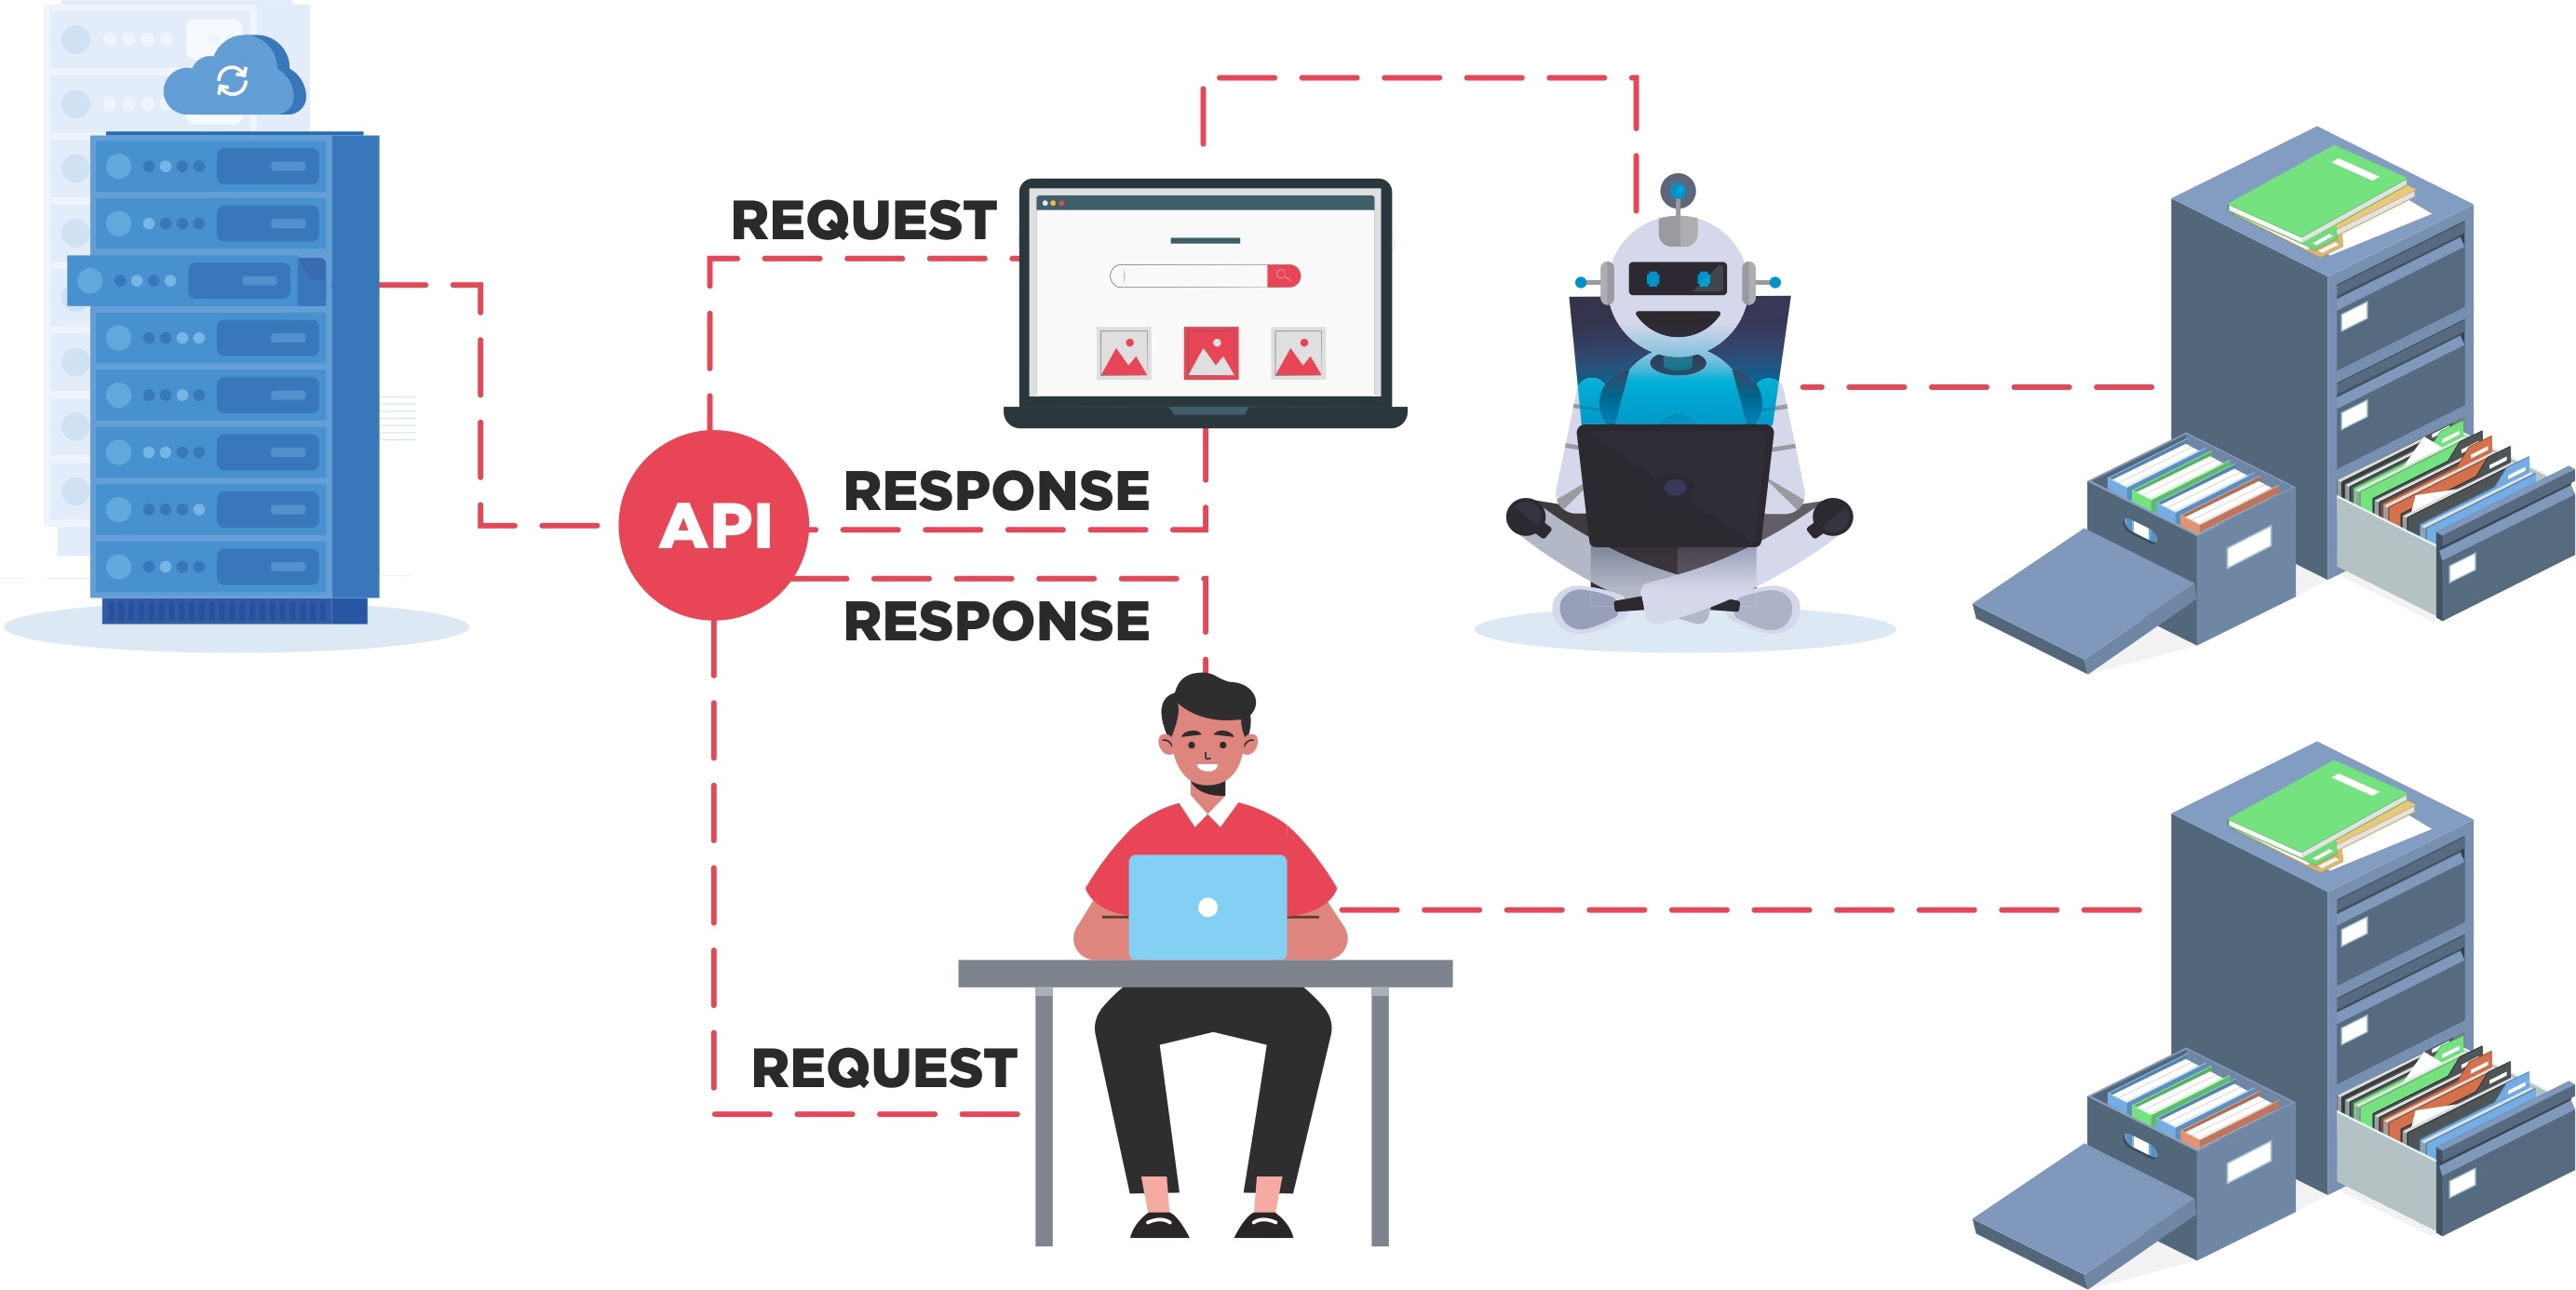
\includegraphics[width = \textwidth]{api.jpg}
   }
   \only<+>{
        \begin{definition}
            \emph{Aplication Programming Interface} is a communication protocol between a client and a server intended to simplify the building of client-side software. In other words, it is a contract between the client and the server which defines the format of possible requests and the format of the response (i.e. format of the data).
        \end{definition}
   }
   \only<+>{
      \framesubtitle{GDELT API}
      \begin{enumerate}
         \item Read the documentation
         \item Test the API in the web browser
         \item Extract the data using BigQuery
         \item Analyze the data
      \end{enumerate}
   }
\end{frame}


\end{document}